% This must be in the first 5 lines to tell arXiv to use pdfLaTeX, which is strongly recommended.
\pdfoutput=1
% In particular, the hyperref package requires pdfLaTeX in order to break URLs across lines.

\documentclass[11pt]{article}

\usepackage[a4paper, total={6in, 8in}]{geometry}
\usepackage{lineno}
\linenumbers

\usepackage{caption,subcaption}

\usepackage{mystyle}

\usetikzlibrary{calc,patterns,angles,quotes}    
\usetikzlibrary{decorations.pathmorphing}
\tikzset{snake it/.style={decorate, decoration=snake}}

\usepackage{natbib}
\bibliographystyle{abbrvnat}
\usepackage{hyperref}

% Standard package includes
\usepackage{times}
\usepackage{latexsym}

% For proper rendering and hyphenation of words containing Latin characters (including in bib files)
\usepackage[T1]{fontenc}
% For Vietnamese characters
% \usepackage[T5]{fontenc}
% See https://www.latex-project.org/help/documentation/encguide.pdf for other character sets

% This assumes your files are encoded as UTF8
\usepackage[utf8]{inputenc}


\title{An Introduction to an Application of the Implicit Function Theorem}

\author{Justin Chiu \\
  Cornell Tech \\
  \texttt{jtc257@cornell.edu}}

\begin{document}
\maketitle
\begin{abstract}
Gradient-based learning forms the foundation of modern machine learning,
and automatic differentiation allows ML practitioners to easily compute gradients.
While automatic differentiation only costs a constant multiple of the time and space
required to evaluate a function, it has its limitations.
In particular, when evaluating a function itself is expensive,
the direct application of automatic differentiation is infeasible.
In this report, we review the implicit function theorem (IFT)
and its use in reducing the cost of computing gradients in scenarios where
function evaluation is expensive,
focusing on the application of implicit differentiation to variational inference.
\end{abstract}

\section{Introduction}
\label{sec:intro}
Gradient-based learning underpins many of the recent successes in machine learning,
particularly advances involving neural networks.
The key to the success of gradient-based methods is automatic differentiation (AD),
which has greatly increased the development speed of machine learning research by
allowing practitioners to circumvent the error-prone and time-consuming process
of computing gradients manually.
AD operates by reducing functions into compositions of atomic operations,
for which we have a library of derivatives for,
and composing those derivatives via the chain rule.
(introduce the representation of functions as evaluation procedures / computational graphs,
following \citet{griewank2008autodiff})
While efficient relative to the evaluation of the function in question,
taking only a multiplicative constant longer than the evaluation itself,
this may be prohibitively expensive if the original function evaluation itself is costly.
An example of this is if the function takes the form of an unrolled loop,
a common artifact of iterative methods.
As naive AD requires storing all of the intermediate values at each point,
storing the output of all computations at every iteration of a loop can quickly
become infeasible due to memory limitations.

There are a variety of methods for overcoming the space limitations of AD,
of which we only mention three: checkpointing, reversible computation, and implicit differentiation.
A first method, checkpointing, improves space complexity at the cost of time.
Rather than storing all intermediate computation,
checkpointing instead recomputes values when needed.
This can result in a large slowdown,
and also requires careful choosing of which computationals subgraphs to checkpoint.
A second method is an improvement upon checkpointing, called reversible computation \citep{maclaurin2015reversible,gomez2017reversible},
which improves space complexity at the cost of expressivity, but not speed.
Reversible computation ensures that the gradient with respect to (wrt) input depends only on the output,
allowing the input to be discarded during function evaluation.
This is typically accomplished by ensuring that the input is easily reconstructed from the output,
restricting the expressivity of layers.
A third method is implicit differentiation,
which potentially improves space complexity at the cost of stronger assumptions.
Implicit differentiation relies on the implicit function theorem (IFT),
which gives conditions under which derivatives can be computed independent of
intermediate computation.
The primary condition is the characterization of the output as the solution
to a series of equations.

In this report, we will cover the use of the implicit function theorem
in OptNet \citep{optnet}, which allows us to use the output of an
optimization problem inside a neural network.
{\color{red} Explain OptNet}
%and apply it to reducing the computational cost of taking derivatives through variational inference.

\paragraph{Bilevel Optimization}
One application of implicit differentiation is bilevel optimization.
Bilevel optimization problems are, as implied by the name,
optimization problems with another nested inner optimization problem embedded within.
Methods for solving bilevel optimization typically proceed iteratively.
For every iteration when solving the outer optimization problem,
we must additionally solve an inner optimization problem.

The application we focus on in this report is expressing individual layers of a neural network declaratively
as the solution of an optimization problem \citep{optnet,agrawal2019diffcvx,gould2019declarative}.
This allows models to learn, without heavy manual specification, the constraints of the problem
in addition to the parameters of the objective.
We will discuss this in further detail later on in the report,
when we go over OptNet \citep{optnet}.

Other applications that can be formulated as bilevel optimization problems are
hyperparameter optimization, metalearning, and variational inference.
Hyperparameter optimization formulates hyperparameter tuning, such as the shrinkage penalty in Lasso,
as a bilevel optimization problem by computing gradients wrt the penalty through the entire learning procedure
of the linear model \citep{lorraine2019implasso}.
(Other works on hyperparam opt \citep{maclaurin2015reversible,bertrand2020implicit})
Similarly, metalearning learns the parameters of a model such that the model is able to quickly
be adapted to a new task via gradient descent \citep{finn2017maml,rajeswaran2019imaml}.
This is accomplished by differentiating through the learning procedure of each new task.
Finally, a variant of variational inference follows a very similar format:
semi-amortized variational inference (SAVI) aims to learn a model that is able to provide
a good initialization for variational parameters that are subsequently updated
to maximize a lower bound objective \citep{kim2018savi}.
This is also accomplished by differentiating through the iterative optimization procedure
applied to the variational parameters during inference.
(Other VI papers \citep{vi,johnson2017pgm})

{\color{red} finish loop, how does IFT help with these applications}

\section{The Implicit Function Theorem}
The implicit function theorem (IFT) has a long history, as well as many applications
in a wide variety of fields such as economics and differential geometry.
For an overview of the history of the IFT and some of its classical applications
in mathematics and economics,
see the book by \citet{iftbook}.

\subsection{What is the IFT?}
Consider the unit circle,
governed by the relation $F(a,b) = a^2 + b^2 - 1 = 0$,
which can be interpreted as a system of equations.
As $F$ fails the vertical line test, we cannot write $b$ as a function of $a$ globally.
This prevents us from taking derivatives, for example $\frac{db}{da}$.
However, we can use local parameterizations: $f_1(a) = \sqrt{1-b^2}$ if $b > 0$
or $f_2(a) = -\sqrt{1-b^2}$ if $b<0$.
These local parameterizations then allow us to take derivatives $\frac{db}{da}$
at particular points $(a,b)$ using the corresponding parameterization.
See Fig.~\ref{fig:circle} for an illustration.
The IFT generalizes this example, and formalizes the conditions under which there exist
smooth local parameterizations for a given relation or system of equations.
Unlike in this example, the IFT does not give those local parameterizations.
It only gives the derivatives, leaving the local functions implicit,
hence the `implicit' in IFT.

\begin{figure}
\centering
\begin{subfigure}[b]{0.45\textwidth}
\centering
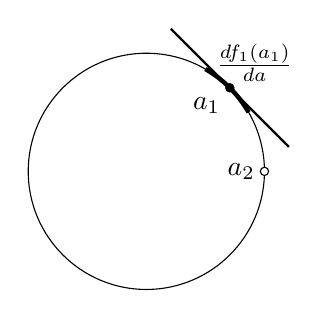
\begin{tikzpicture}[scale=.75]
\draw (0,0) circle (2);

\node at ($2*({sqrt(2) / 2}, {sqrt(2) / 2})$) (x)[below left] {$a_1$};
\draw[fill=black] ($2*({sqrt(2) / 2}, {sqrt(2) / 2})$) circle (2pt);

% neighbourhood 
\draw[ultra thick] ($2*({sqrt(2) / 2}, {sqrt(2) / 2})$) arc(45:60:2);
\draw[ultra thick] ($2*({sqrt(2) / 2}, {sqrt(2) / 2})$) arc(45:30:2);


% tangent
%\path (2,1) node[point,label={180:P}] {P} at +(120:2){};
\node at ($2*({sqrt(2) / 2 + .21}, {sqrt(2) / 2 + .21})$) {$\frac{df_1(a_1)}{da}$};
\draw[thick] ($2*({sqrt(2) / 2 + -.5}, {sqrt(2) / 2 + .5})$) --
    ($2*({sqrt(2) / 2 + .5}, {sqrt(2) / 2 -.5})$);

% singular point
\node at (2,0) (x2)[left] {$a_2$};
\draw[fill=white] (2,0) circle (2pt);
\end{tikzpicture}
\caption{}
\end{subfigure}
%\hspace{1em}
\begin{subfigure}[b]{0.45\textwidth}
\centering
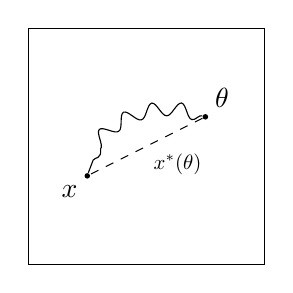
\begin{tikzpicture}[scale=.75]
%\draw (0,0) circle (2);
\draw (-2,-2) rectangle (2,2);

\node[circle,fill=black, minimum size=2pt, inner sep=0] (x) at (1,.5) {};
\node at (x)[above right] {$\theta$};
\node[circle,fill=black, minimum size=2pt, inner sep=0] (y) at (-1,-.5) {};
\node at (y)[below left] {$x$};

\draw[snake it] (x)      to [bend right = 45] (y);
\path[dashed] (x) edge (y) node[midway,below right]{$x^*(\theta)$};

\end{tikzpicture}
\caption{}
\end{subfigure}
\caption{
\label{fig:circle}
Illustration (a) contains circle, defined by the relation $a^2 + b^2 - 1 = 0$.
While we cannot differentiate the relation directly,
we can compute derivatives at the point $a_1$ using the local parameterization $f_1(a)=\sqrt{1-b^2}$ that holds
in a neighbourhood around $a_1$.
We cannot use the same parameterization at $a_2$ as the derivative is undefined.
Separately, illustration (b) shows an example relationship between the parameters $\theta$,
solution $x$, and implicit function $x^*(\theta)$ of the IFT.
The rectangle depicts a space which, in this example,
contains both $\theta$ and $x$.
This is not necessary for the IFT, but simplifies illustration.
The parameters $\theta$ provide an initial point, which is then iteratively refined
into solution $x$, shown by the curved line.
If $x$ satisfies the conditions of the IFT, then the IFT guarantees the
existence of the implicit solution mapping $x^*(\theta)$,
and tells us how to compute $\frac{dx^*(\theta)}{d\theta}$.
This is useful if the iterative procedure (squiggly line), is too expensive
to store in memory for use in automatic differentiation.
}
\end{figure}


%% MINIPAGE
\begin{figure}
\begin{minipage}{0.48\textwidth}
\centering
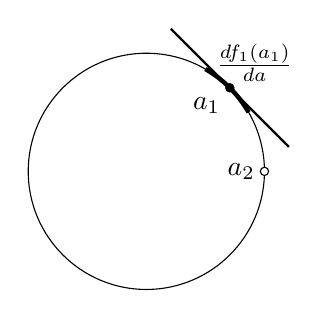
\begin{tikzpicture}[scale=.75]
\draw (0,0) circle (2);

\node at ($2*({sqrt(2) / 2}, {sqrt(2) / 2})$) (x)[below left] {$a_1$};
\draw[fill=black] ($2*({sqrt(2) / 2}, {sqrt(2) / 2})$) circle (2pt);

% neighbourhood 
\draw[ultra thick] ($2*({sqrt(2) / 2}, {sqrt(2) / 2})$) arc(45:60:2);
\draw[ultra thick] ($2*({sqrt(2) / 2}, {sqrt(2) / 2})$) arc(45:30:2);


% tangent
%\path (2,1) node[point,label={180:P}] {P} at +(120:2){};
\node at ($2*({sqrt(2) / 2 + .21}, {sqrt(2) / 2 + .21})$) {$\frac{df_1(a_1)}{da}$};
\draw[thick] ($2*({sqrt(2) / 2 + -.5}, {sqrt(2) / 2 + .5})$) --
    ($2*({sqrt(2) / 2 + .5}, {sqrt(2) / 2 -.5})$);

% singular point
\node at (2,0) (x2)[left] {$a_2$};
\draw[fill=white] (2,0) circle (2pt);
\end{tikzpicture}
\caption{
\label{fig:circle2}
A circle, defined by the relation $a^2 + b^2 - 1 = 0$.
While we cannot differentiate the relation directly,
we can compute derivatives at the point $a_1$ using the local parameterization $f_1(a)=\sqrt{1-b^2}$ that holds
in a neighbourhood around $a_1$.
We cannot use the same parameterization at $a_2$ as the derivative is undefined.}
\end{minipage}
\hfill
\begin{minipage}{0.48\textwidth}
\centering
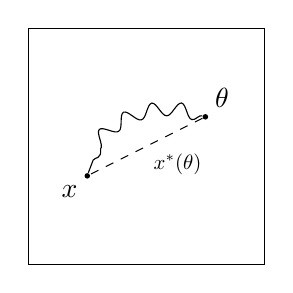
\begin{tikzpicture}[scale=.75]
%\draw (0,0) circle (2);
\draw (-2,-2) rectangle (2,2);

\node[circle,fill=black, minimum size=2pt, inner sep=0] (x) at (1,.5) {};
\node at (x)[above right] {$\theta$};
\node[circle,fill=black, minimum size=2pt, inner sep=0] (y) at (-1,-.5) {};
\node at (y)[below left] {$x$};

\draw[snake it] (x)      to [bend right = 45] (y);
\path[dashed] (x) edge (y) node[midway,below right]{$x^*(\theta)$};

\end{tikzpicture}
\label{fig:a}
\caption{
An example relationship between the parameters $\theta$,
solution $x$, and implicit function $x^*(\theta)$ of the IFT.
The rectangle depicts a space which, in this example,
contains both $\theta$ and $x$.
This is not necessary for the IFT, but simplifies illustration.
The parameters $\theta$ provide an initial point, which is then iteratively refined
into solution $x$, shown by the curved line.
If $x$ satisfies the conditions of the IFT, then the IFT guarantees the
existence of the implicit solution mapping $x^*(\theta)$,
and tells us how to compute $\frac{dx^*(\theta)}{d\theta}$.
This is useful if the iterative procedure (squiggly line), is too expensive
to store in memory for use in automatic differentiation.
}
\end{minipage}
\end{figure}

Formally, the IFT gives sufficient conditions under which the solution $x\in\R^m$
to a system of equations, $F(\theta, x) = 0$ with $F: \R^n\times\R^m\to\R^m$,
can locally be written as a function of just the parameters $\theta\in\R^n$,
i.e. there exists a solution mapping $x^*:\R^n\to\R^m$
in the neighbourhood of the particular point $(\theta,x)\in\dom(F)$.
These conditions are as follows:
\begin{enumerate}
\item We have a solution point $(\theta, x)$ that satisfies the system of equations
    $F(\theta, x) = 0$.
\item $F$ has at least continuous first derivatives: $F \in \mcC^k$.
\item The Jacobian of $F$ wrt $x$ evaluated at the solution point $(\theta,x)$ is nonsingular:
    $\det \frac{d F}{d x} \neq 0$.
\end{enumerate}
Given these conditions hold for $F,\theta,$ and $x$, we are then
able to assert the existence of the implicit solution mapping $x^*(\theta)$,
and determine its derivative
$\frac{d x^*(\theta)}{d\theta} = -[\frac{dF(\theta,x)}{dx}]^{-1}
    \frac{d F(\theta,x)}{d\theta}$.
We provide an illustration in Fig.~\ref{fig:circle}.

\subsection{Why is the IFT useful?}
As mentioned in Sec.~\ref{sec:intro}, the IFT is useful for saving memory when performing
automatic differentiation.
The main benefit of the IFT is that once we have a solution to a system of equations,
we can forget about how we obtained that solution but still compute derivatives.

As an example, say we obtained a solution using gradient descent,
which from an initial point $\theta = x_0$
produces $x_1, x_2, ..., x_{1000}$ if you run it for 1000 iterations.
Without the IFT, you would have to store all 1000 $x$'s
and the computation used to produce them.
The IFT lets you throw away $x_1$ through $x_{999}$, and gives you the derivative
$\frac{dx_{1000}}{dx_0}$.

In particular, we will show how to compute derivatives of the solution of an optimization problem
wrt parameters of the problem without storing intermediate computations.
We will use the optimality criteria of the optimization problem to define a system of equations,
then apply the IFT to compute the Jacobian of the solution wrt the parameters.
This methodology allows us to use the solution to an optimization problem
as the output of a layer within a neural network,
as done in OptNet \citep{optnet}.
%We will then discuss the problem addressed by this method in OptNet.

Afterwards, we will cover an application of the IFT to speeding up variational inference.

\section{Embedding Optimization inside a Neural Network}
As an introductory example,
we will replace the softmax layer of a neural network with an equivalent function
defined as the output of an optimization problem, then derive derivatives using the IFT.
We will start by reviewing softmax and its expression as an optimization problem.
After checking the conditions of the IFT hold, we can then compute derivatives.
Since the Jacobian of softmax is known, we can directly verify that the IFT gives
the correct answer.

\subsection{The Chain Rule}
Before we get into the details of softmax, we first setup the learning problem.
We are interested in training a neural network model that consists of stacks of layers,
all of which take the output of the previous layer as input.
In order to train such a model we rely on backpropagation,  also known as reverse mode AD.
Reverse mode AD propagates error information backward through the network via the chain rule
for computing derivatives of composite functions.
Key to this process is the Jacobian matrix of each layer, the matrix of partial derivatives
of the layer's outputs wrt its inputs.

As an example, let's say we would like to maximize $b = f_3(f_2(f_1(a)))$ with a gradient-based method,
where $b\in\R$; $f_3:\R^n\to\R$; $f_1,f_2:\R^n\to\R^n$; and $a\in\R^n$.
We can compute the derivatives of $b$ wrt each layer via the chain rule.
Focusing on the first layer $f_1$,
we have $\frac{db}{df_1} = \frac{db}{df_3}\frac{df_3}{df_2}\frac{df_2}{df_1}$,
where each term is the Jacobian matrix for the respective layer in the denominator.
These derivatives can then be used to update the parameters of each layer,
completing one iteration of the learning process.

Given its key role in learning, we will proceed towards computing the Jacobian of softmax
using the IFT by first reviewing softmax.

\subsection{Softmax}
Softmax is often used to parameterize categorical distributions within neural networks,
such as in attention layers.
It has its origins in statistical mechanics and decision theory, and functions
as a differentiable surrogate for argmax.

Softmax assumes that we have $n$ items with independent utilities, $\theta \in \R^n$,
which indicate preferences.
Softmax then gives the following distribution over items:
$x_i = \frac{\exp(\theta_i)}{\sum_j \exp(\theta_j)}$, with $x\in\R^n$.
Interestingly, softmax arises as the solution of an optimization problem
\citep{gao2018properties}.

The output of softmax is the solution of the following optimization problem:
\begin{equation}
\label{eqn:softmax-opt}
\begin{aligned}
\textrm{maximize } \quad & x^\top\theta + H(x)\\
\textrm{subject to } \quad & x^\top \mathbf{1} = 1\\
& x \succeq 0,
\end{aligned}
\end{equation}
where $H(x) = -\sum_i x_i \log x_i$ is the entropy.
This corresponds to an entropy-regularized argmax optimization problem.
We will refer to this as the softmax problem.

Our goal is to compute the Jacobian of softmax
$\frac{dx}{d\theta} = \frac{d\softmax(\theta)}{d\theta}$
using the IFT and the optimization problem above.
This would allow us to compute gradients via autodiff inside a
neural network via the chain rule,
although we will stop at computing the Jacobian.
While this is not of practical use (there is a closed-form equation
for both softmax and its Jacobian),
we use it as an introduction to the mechanism
behind OptNet (and other differentiable optimization layers)
\citep{optnet,agrawal2019diffcvx}.
Applying the IFT to optimization problems consists of four steps:
\begin{enumerate}
\item Find a solution to the optimization problem.
\item Write down the system of equations.
\item Check that the conditions of the IFT hold.
\item Compute the derivative of the implicit solution mapping wrt the parameters.
\end{enumerate}

We assume the first step has been done for us,
and we have some solution $x$ to the softmax problem.
We will then use the IFT to compute gradients of $x$ wrt the parameters $\theta$
by following the rest of the steps.

\subsection{The KKT conditions determine $F$}
Given an optimization problem, the KKT conditions determine a system of equations
that the solution must satisfy \citep{kkt-thesis,kkt}.
We will use the KKT conditions of the softmax problem in
Eqn.~\ref{eqn:softmax-opt} to determine the function $F$ in the IFT.

First, we introduce dual variables $u\in\R,v\in\R^n$ and write out the Lagrangian:
$$\mcL(\theta, x, u, v) = x^\top\theta + H(x) + u(x^\top \mathbf{1} - 1) + v^\top x.$$
We include $u,v$ as solution variables.
We then have the following necessary conditions for a solution $(x,u,v)$,
i.e. the KKT conditions:
\begin{equation}
\begin{aligned}
\nabla_x \mcL(\theta, x,u,v) = 0 && \textrm{(stationarity)}\\
u(x^{\top} \mathbf{1} - 1) = 0 && \textrm{(primal feasibility)}\\
\diag(v)x = 0 && \textrm{(complementary slackness)}\\
v \succeq 0 && \textrm{(dual feasibility)}
\end{aligned}
\end{equation}
As we are interested in the primal variable or solution $x$,
we focus on the first three conditions.

In full, the system of equations $F(\theta, x,u,v) = 0$ is
\begin{equation}
\label{eqn:system}
\begin{aligned}
\theta + -\log(x) - 1 + u\mathbf{1} + v &= 0\\
u(x^{\top} \mathbf{1} - 1) &= 0\\
\diag(v)x &= 0.
\end{aligned}
\end{equation}

Now we can check the conditions of the IFT.
Any solution $(x,u,v)$ will satisfy $F(\theta, x,u,v) = 0$,
and $F \in \mcC^1$.
All that remains is to check that the Jacobian matrix of $F$ is non-singular.

The Jacobian $\frac{dF}{d(x,u,v)}\in\R^{n\times n+1+n}$ is given by
\begin{equation}
\label{eqn:f-jac}
\frac{dF}{d(x,u,v)}=
\begin{bmatrix}
\diag(x)^{-1} & -\mathbf{1} & -I_n \\
u\mathbf{1}^\top & x^\top\mathbf{1} - 1 & 0\\
\diag(v) & 0 & \diag(x)
\end{bmatrix}.
\end{equation}
Since a solution must be feasible, we know that $x^\top\mathbf{1} = 1$ and $u > 0$.
With the additional information that the domain of $H(x)$
adds the implicit constraint that $\forall i, x_i > 0$,
we can deduce that the Jacobian of $F$ is full rank and therefore has nonzero determinant.
This shows that the conditions of the IFT hold.


\subsection{The Jacobian of Softmax}
Now that we have shown that the conditions of the IFT hold,
we can proceed to apply the second part of the IFT in order to compute $\frac{dx}{d\theta}$.
The second part of the IFT tells us that we can compute the Jacobian of the
solution mapping $\frac{d(x,u,v)}{d\theta} = \frac{dx^*(\theta)}{d\theta}
= \left[\frac{dF}{d(x,u,v)}\right]^{-1}\frac{dF}{d\theta}$,
then pick out the relevant components.

The second term, $\frac{dF}{d\theta}$, is simple.
Since $\theta$ only appears in the first vector-valued function of $F$
(see Eqn.~\ref{eqn:system}), we have
\begin{equation}
\label{eqn:df-dtheta}
\frac{dF}{d\theta} = \begin{bmatrix}
    I_n\\
    0
\end{bmatrix}.
\end{equation}
The large amount of sparsity allows us to skip some computation further down.

Next, we have to invert the Jacobian from Eqn.~\ref{eqn:f-jac}:
\begin{equation}
\label{eqn:dsystem-matrix}
\left[\frac{dF}{d(x,u,v)}\right]^{-1} = \begin{bmatrix}
\diag(x)^{-1} & -\mathbf{1} & -I_n \\
u\mathbf{1}^\top & x^\top\mathbf{1} - 1 & 0\\
\diag(v) & 0 & \diag(x)
\end{bmatrix}^{-1}.
\end{equation}
We use the block-wise inversion formula
\begin{equation*}
\begin{bmatrix}
A & B\\
C & D
\end{bmatrix}^{-1} = \begin{bmatrix}
    (A - BD^{-1}C)^{-1} & 0\\
    0 & (D - CA^{-1}B)^{-1}
\end{bmatrix}
\begin{bmatrix}
    I & -BD^{-1}\\
    -CA^{-1} & I
\end{bmatrix},
\end{equation*}
where
\begin{align*}
A = \begin{bmatrix} \diag(x)^{-1} & -\mathbf{1} \\ u\mathbf{1}^\top & 0 \end{bmatrix}&\qquad\qquad
B = \begin{bmatrix}-I_n \\ 0\end{bmatrix}\\
C = \begin{bmatrix}\diag(v) & 0\end{bmatrix} &\qquad\qquad
D = \diag(x).
\end{align*}
However, by complementary slackness, we have $v = 0$, reducing the above to
\begin{equation*}
\begin{bmatrix}
A & B\\
C & D
\end{bmatrix}^{-1} = \begin{bmatrix}
    A^{-1} & 0\\
    0 & D^{-1}
\end{bmatrix}
\begin{bmatrix}
    I & -BD^{-1}\\
    0 & I
\end{bmatrix}.
\end{equation*}
As we are interested in computing $\frac{dx}{d\theta}$,
rather than the full derivative $\frac{d(x,u,v)}{d\theta}$,
in addition to the sparsity of $\frac{dF}{d\theta}$, 
we only have to solve for the upper-left $n\times n$ block of $A^{-1}\in\R^{n+1\times n+1}$.
To do so, we will repeat the same block-wise inverse computation.
Let us denote $A = \begin{bmatrix}E & F \\ G & H\end{bmatrix}$.
First, we compute the Schur complement of $A$,
\begin{equation}
A/E = H - GE^{-1}F = 0 + u\mathbf{1}^\top\diag(x)\mathbf{1} = ux^\top\mathbf{1}.
\end{equation}
Since $x$ is feasible, we have $A/E = u$ due to the equality constraints
($x$ must sum to 1 as a probability mass function).
Then, we have
\begin{equation}
A^{-1} = \begin{bmatrix}
\diag(x)^{-1} & -\mathbf{1}\\
u\mathbf{1}^\top & 0
\end{bmatrix}^{-1}
=\begin{bmatrix}E & F \\ G & H\end{bmatrix}^{-1}
= \begin{bmatrix}
E^{-1} + E^{-1}F(A/E)^{-1}GE^{-1} & -E^{-1}F(A/E)^{-1}\\
-(A/E)^{-1}GE^{-1} & (A/E)^{-1}
\end{bmatrix}.
\end{equation}
Plugging in, we have
\begin{equation}
\begin{aligned}
A^{-1} 
&= \begin{bmatrix}
\diag(x) - \diag(x)\mathbf{1}u^{-1}u\mathbf{1}^\top\diag(x)
    & \diag(x)\mathbf{1}u^{-1}\\
-u^{-1}u\mathbf{1}^\top \diag(x) & u^{-1}
\end{bmatrix}\\
&= \begin{bmatrix}
\diag(x) - xx^\top
    & u^{-1}x\\
    -x^\top & u^{-1}
\end{bmatrix}.
\end{aligned}
\end{equation}
Pulling out the top-left $n\times n$ block yields
the Jacobian $\frac{d x}{d\theta} = \diag(x) - xx^\top$,
which agrees with directly differentiating softmax \citep{sparsemax}.

With this, we have shown that we can rewrite softmax as an optimization problem,
and differentiate the solution of that problem wrt the parameters in a solver-agnostic
manner.

%(Example showing build-up of memory from reversible SGD vs IFT would be nice here,
%ie code it up and plot memory consumption / speed. maybe not best example though)

\subsection{Limitations}
In order to compute the derivative $\frac{dx}{d\theta}$, we had to invert the Jacobian of $F$.
However, The first part of $F$ (recall from Eqn.~\ref{eqn:system}), the stationarity condition $\nabla_x\mcL = 0$,
already involved the Jacobian of the Lagrangian $\mcL$.
In general, this means that in order to apply the IFT to solutions of optimization problems,
we must compute the inverse Hessian (or at least a Hessian-vector-product).
The Hessian is a matrix of size $O(n^2)$, and inverting this would take $O(n^3)$ computation.
Thankfully, there are relatively cheap ways of approximating this computation,
such as with approximate (inverse) Hessian-vector-product techniques
\citep{rajeswaran2019imaml,lorraine2019hoift}.

\subsection{Extensions}
The methods we covered can be extended to variations of argmax problems
other than the softmax problem.
The softmax problem relaxed the argmax problem by introducing entropy regularization.
Rather than regularizing with entropy, one could instead alter the objective to find
the Euclidean projection of the parameters onto the probability simplex,
resulting in SparseMax \citep{sparsemax}.
While the output of softmax variants often have a closed form expression,
the IFT provides another way of deriving their Jacobians
and could potentially pave the way for generalizations.

More generally, the IFT can be applied to cases where, unlike softmax,
we do not have an explicit functional form (i.e., the unit circle),
and outputs are governed only by a system of equations.
This includes more general optimization problems, such as quadratic programs \citep{optnet}
or other convex optimization problems \citep{agrawal2019diffcvx},
as well as the solutions of differential equations \citep{neuralode}.

\section{OptNet}
OptNet generalizes the methodology applied above to the softmax problem by
including parameterized constraints and computing the gradients of the solution
wrt all parameters.
This allows us to learn not only the objective, but also the constraints.
Constraint learning allows models with optimization layers to perform well
on tasks with hard constraints, such as learning to play
Sudoku from only inputs and outputs \citep{optnet}.

\subsection{Quadratic Programs}
OptNet applies the IFT to quadratic programs (QPs) in particular.
As one of the first attempts to apply the IFT to differentiable optimization layers in
neural networks, OptNet targeted QPs due to their status
as the simplest nonlinear optimization problem (speculation).
The methodology remains the same as the softmax problem:
given a QP and a solution,
use the KKT conditions to produce a system of equations then apply the IFT
/ implicit differentiation to compute the derivative of the solution wrt the
parameters of the objective and constraints.

Quadratic programs take the following form:
\begin{equation}
\label{eqn:qp}
\begin{aligned}
\textrm{maximize } \quad & \frac12 x^\top Q x + q^\top x\\
\textrm{subject to } \quad & Ax = b\\
& Gx \leq h,
\end{aligned}
\end{equation}
where we optimize over $x$ and the parameters are $\theta = \set{Q, q, A, b, G, h}$.
Compared to the softmax problem in Eqn.~\ref{eqn:softmax-opt},
we see that the main difference is just the learnable parameters in the constraints.
As the application of the IFT is almost identical, we will not cover it in detail.

The second contribution of OptNet was the extension of a state-of-the-art interior point
solver \citep{optnet}, and its adaptation to parallel machines (GPUs) and batch processing.
While outside the scope of this report, see the paper by \citet{optnet} for the details.

\section{Semi-Amortized Variational Inference (POSTPONED)}
We now apply the IFT to variational inference.

Variational inference has found success in recent applications to generative models,
in particular by allowing practitioners to depart from conjugate models
and extend emission models with expressive neural network components.
The main insight that led to this development is that inference can be amortized through
the use of an inference network.
One approach to variational inference, stochastic variational inference (SVI),
introduces local, independent variational parameters for every instance of hidden variable.
While flexible, the storage of all variational parameters is expensive, and the optimization
of each parameter independently slow \citep{}.
Amortized variational inference (AVI) solves that by instead using a hierarchical process.
Variational parameters are produced hierarchically via an inference network,
which in turn generates the local variational parameters \citep{}.
The resulting local parameters may or may not be subsequently optimized.

Failure to further optimize local variational parameters may result in an amortization gap \citep{}.
Prior work has shown that this gap can be ameliorated by performing a few steps of
optimization on the generated local parameters obtained from the inference network,
and even by propagating gradients through the optimization process.
Optimizing through the inner optimization problem results in semi-amortized variational inference
(SAVI) \citep{}.

As our main motivating example, we will examine whether we can apply the IFT to SAVI.
We will start by formalizing the problem of variational inference for a simple model.

We will start with a model defined by the following generative process,
used by \citet{dai2020vae} to analyze posterior collapse:
\begin{enumerate}
\item Choose a latent code from the prior distribution $z \sim p(z) = N(0, I)$.
\item Given the code, choose an observation from the emission distribution
    $x \mid z \sim p_\theta(x \mid z) = N(\mu_x(z, \theta), \gamma I)$,
\end{enumerate}
where $\mu_x(z, \theta) \equiv \MLP(z, \theta)$ and $\gamma > 0$ is a hyperparameter.
This yields the joint distribution $p(x,z) = p(x\mid z)p(z)$.

Since the latent code $z$ is unobserved, training this model would require optimizing the
evidence $p(x) = \int p(x,z)$.
However, due to the MLP parameterized $\mu_x$, the integral is intractable.
Variational inference performs approximate inference by introducing variational distribution
$q_\phi(z \mid x)$ and maximizing the following lower bound on $\log p(x)$:
\begin{equation}
    \log p(x) - \KL{q(z \mid x) || p(z \mid x)}
    = \Es{q_\phi(z \mid x)}{\log \frac{p_\theta(x,z)}{q_\phi(z\mid x)}} = L(\theta, \phi).
\end{equation}

(Write out objective in full.)

While SVI introduces local parameters for each instance of $z$,
and AVI uses a single $q(z \mid x)$ for all instances,
we will follow the approach of SAVI.
We will perform inference as follows:
For each instance $x$, produce local variational parameter
$z^{(0)} = g(x; \phi)$.
Obtain $z^*$ by solving $\mcL(\theta, z^{(0)}) = 2$, with (local) optima $\ell^*$.
Take gradients through the whole procedure,
i.e. compute $\frac{\partial \ell^*}{\partial \phi}
= \frac{\partial\ell^*}{\partial z^*}\frac{\partial z^*}{\partial z^{(0)}}
\frac{\partial z^{(0)}}{\partial \lambda}$.
The main difficuty lies in computing $\frac{\partial z^*}{\partial z^{(0)}}$.
(Highlight challenge)

In order to avoid the memory costs of storing all intermediate computation performed
in a solver, we will instead apply the IFT.
In order to apply the IFT, we must satisfy the three conditions.
First, we must have a solution point to a system of equations, $F(x_0, z_0) = 0$.
In this setting, we will use the KKT conditions of the optimization problem to define $F$.

\section{Limitations}

\bibliography{bib}

\appendix

\section{Example Appendix}
\label{sec:appendix}

Neural ODEs use reversibility.

\end{document}
